\documentclass[11pt]{article}

\usepackage[a4paper,margin=1in]{geometry}
\usepackage[T1]{fontenc}
\usepackage{amsmath,amssymb}
\usepackage{graphicx}
\usepackage{booktabs}
\usepackage{multirow}
\usepackage{float}
\usepackage{xcolor}
\usepackage{hyperref}

\graphicspath{{../temp_analysis/}{../results/}}
\hypersetup{colorlinks=true, linkcolor=blue!50!black, urlcolor=blue!50!black}

\title{Ha senso addestrare un MLP su una stima di Parzen?\\
\large Indagine sperimentale sul vantaggio dell'approccio (caso monovariato)}
\author{Progetto parzen-cdf}
\date{\today}

\begin{document}
\maketitle

\begin{abstract}
La pipeline del progetto addestra un percettrone multistrato (MLP) sigmoidale a regredire la funzione
di ripartizione (CDF) stimata con finestre di Parzen logistiche, usando come etichette il valore di
Parzen nei soli punti campionati, e ricava la densita' per derivazione della rete. In una dimensione
la rete eguaglia il proprio bersaglio di Parzen ma non lo supera, e Parzen (o perfino la CDF empirica)
stima gia' bene una CDF. Ci si chiede allora se l'approccio abbia un vantaggio reale. Questo documento
riporta un'indagine sistematica (quindici linee sperimentali con verifica avversariale, piu' ricerca
bibliografica). La conclusione, onesta, e' che l'approccio ha senso, ma \textbf{non come stimatore piu'
accurato}: ha senso come surrogato compatto, valido per costruzione, differenziabile e a costo di
interrogazione costante di una stima di Parzen di cui ci si fida (una distillazione), e come mattone
per il caso multivariato. Un modello addestrato a massima verosimiglianza diretta, quando i dati sono
disponibili, resta piu' accurato.
\end{abstract}

\section{Domanda e metodo}

Tutti gli esperimenti rispettano il vincolo del progetto: la rete si addestra solo sugli $n$ punti
dato, con etichetta $\widehat F(x_i)$ (la CDF di Parzen), e la densita' e' la derivata della rete.
Ogni esperimento e' uno script riproducibile; ogni affermazione e' stata verificata in modo
avversariale da un secondo agente scettico che ne ha ricontrollato o rieseguito i numeri. La metrica
principale e' lo scarto di Kolmogorov-Smirnov (KS) della CDF rispetto alla verita' nota; per la densita'
si usano anche l'errore quadratico medio (MSE), la massa (che deve valere 1) e la frazione di
violazioni di monotonia.

\section{Dove non c'e' vantaggio: l'accuratezza}

Il primo risultato, netto e confermato, e' che l'approccio \emph{non} migliora l'accuratezza in una
dimensione.

\begin{itemize}
  \item \textbf{La rete non batte la migliore Parzen.} Variando la finestra dal nitido al liscio, su
  tre distribuzioni e con rete ben convergente, la migliore rete resta sempre peggiore della migliore
  Parzen (banda oracolo): KS di Parzen $0.014/0.015/0.018$ contro KS della rete $0.018/0.020/0.062$
  (Gaussiana, bimodale, trimodale). La rete e' un regressore \emph{fedele}: non puo' superare il
  maestro che imita.
  \item \textbf{Nessuna maggiore efficienza a pochi campioni.} Per $n \in \{25,50,100,200\}$ la rete
  pareggia sulla Gaussiana e fa peggio sulla bimodale (KS da $-1.4\%$ a $-7.2\%$).
  \item \textbf{Code peggiori.} Parzen vince l'accuratezza nelle code (da circa $2\times$ fino a
  $5$-$20\times$) e raggiunge $0$ e $1$ a precisione macchina; la rete resta a un offset residuo e ha
  una coda di densita' spuriamente spessa.
  \item \textbf{Non puo' battere una KDE, per costruzione.} Un modello a mistura di Gaussiane
  addestrato a massima verosimiglianza batte la rete del $47$-$81\%$ sullo scarto CDF e di $6$-$45$
  volte sull'MSE della densita', pur mantenendo tutti i pregi strutturali. Regredire etichette KDE
  fisse rende la KDE il tetto di accuratezza.
\end{itemize}

\section{Dove il vantaggio e' genuino: la struttura}

\subsection{Validita' gratuita tramite la CDF (il vantaggio piu' netto)}

Imporre i vincoli di una CDF (monotona, in $[0,1]$) e' molto piu' facile e produce sempre un oggetto
valido, rispetto a imporre quelli di una densita' ($\ge 0$, integra a $1$). Confrontando, a parita' di
tutto, la route CDF (rettifica a valle: massimo cumulativo piu' rinormalizzazione) contro una rete che
produce direttamente la densita':

\begin{table}[H]
  \centering
  \caption{Route CDF contro route densita' diretta (MSE della densita', massa).}
  \begin{tabular}{lcc}
    \toprule
    metodo & MSE densita' & massa nativa \\
    \midrule
    \textbf{route CDF (rettificata)} & \textbf{0.0024} & \textbf{1.00000 esatta} \\
    densita' diretta + penalita' di normalizzazione & 0.0175 (circa $7\times$ peggio) & $\approx 1$ (variabile) \\
    densita' diretta + rinormalizzazione a posteriori & 0.0038 (circa $1.6\times$ peggio) & 1.28 prima della correzione \\
    \bottomrule
  \end{tabular}
\end{table}

La massa nativa della route densita' si allontana da $1$ al crescere della difficolta' ($1.11$
Gaussiana, $1.33$ bimodale, $1.40$ trimodale): senza correzioni non e' una densita' valida. Questo e' il
punto sollevato da Magdon-Ismail e Atiya (2002), e si accentua in alta dimensione, dove il
normalizzatore della densita' e' un integrale $d$-dimensionale intrattabile.

\begin{figure}[H]
  \centering
  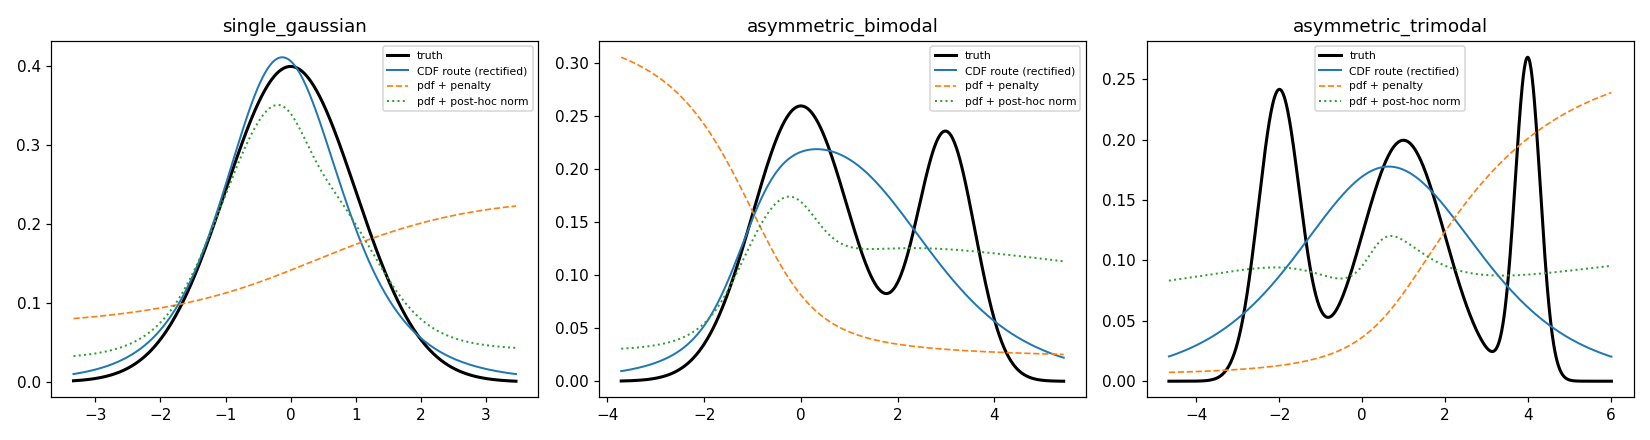
\includegraphics[width=\textwidth]{wf04_pdf_vs_cdf_route.png}
  \caption{Route CDF contro route densita' diretta su tre distribuzioni. La route CDF fornisce una
  densita' valida (massa $1$, non negativa) con maggiore fedelta'; la route diretta o sacrifica la
  forma (penalita') o resta non valida prima di una correzione.}
\end{figure}

\subsection{Ammortamento e compressione}

Il costo di interrogazione della rete e' \emph{costante} nel numero di campioni; quello di Parzen e'
$O(n)$ a ogni interrogazione.

\begin{table}[H]
  \centering
  \caption{Costo di interrogazione (griglia di 1000 punti) e memoria.}
  \begin{tabular}{lcc}
    \toprule
    $n$ & Parzen (query CDF) & rete (query CDF) \\
    \midrule
    1000 & 8.6 ms & \multirow{4}{*}{0.10 ms (costante, 97 parametri)} \\
    5000 & 73.6 ms & \\
    20000 & 298 ms & \\
    100000 & 1173 ms & \\
    \bottomrule
  \end{tabular}
\end{table}

A $n=100000$ la rete e' circa $12000\times$ piu' veloce di una KDE ingenua e comprime la memoria di
circa $1031\times$ ($97$ float contro $n$); i parametri crescono solo di circa $+32$ per dimensione.
\textbf{Limiti onesti}: e' un vantaggio di \emph{servizio}, non di accuratezza; non e' stato
confrontato con le KDE veloci (alberi $k$-d, trasformata di Gauss veloce, KDE binned/FFT) che esistono
proprio per abbattere il costo $O(n)$, quindi la magnitudine e' gonfiata; per una singola
interrogazione Parzen costa meno (nessun addestramento). L'argomento sulla dimensione e' stato
verificato solo fino a $D=3$ su una Gaussiana separabile (MISE relativa che peggiora di circa
$10\times$ per dimensione).

\subsection{Economia di modello tramite copula (Sklar)}

In due dimensioni, decomporre il congiunto in CDF marginali monovariate piu' una copula parametrica
batte la rete congiunta monolitica in tutti i casi provati (ad esempio, Gaussiana con correlazione
$0.6$: scarto $0.056$ contro $0.289$). Quando la famiglia di copula combacia con la verita', l'errore
del modello di copula sui marginali veri e' quasi nullo ($0.0003$): la stima diventa due buoni fit
monovariati piu' un parametro interpretabile. E' un vantaggio \emph{condizionale}: se la dipendenza e'
genuinamente non gaussiana, il pavimento d'errore e' irriducibile e la rete congiunta e' poco dietro.

\section{Capacita' reali ma non uniche}

\begin{figure}[H]
  \centering
  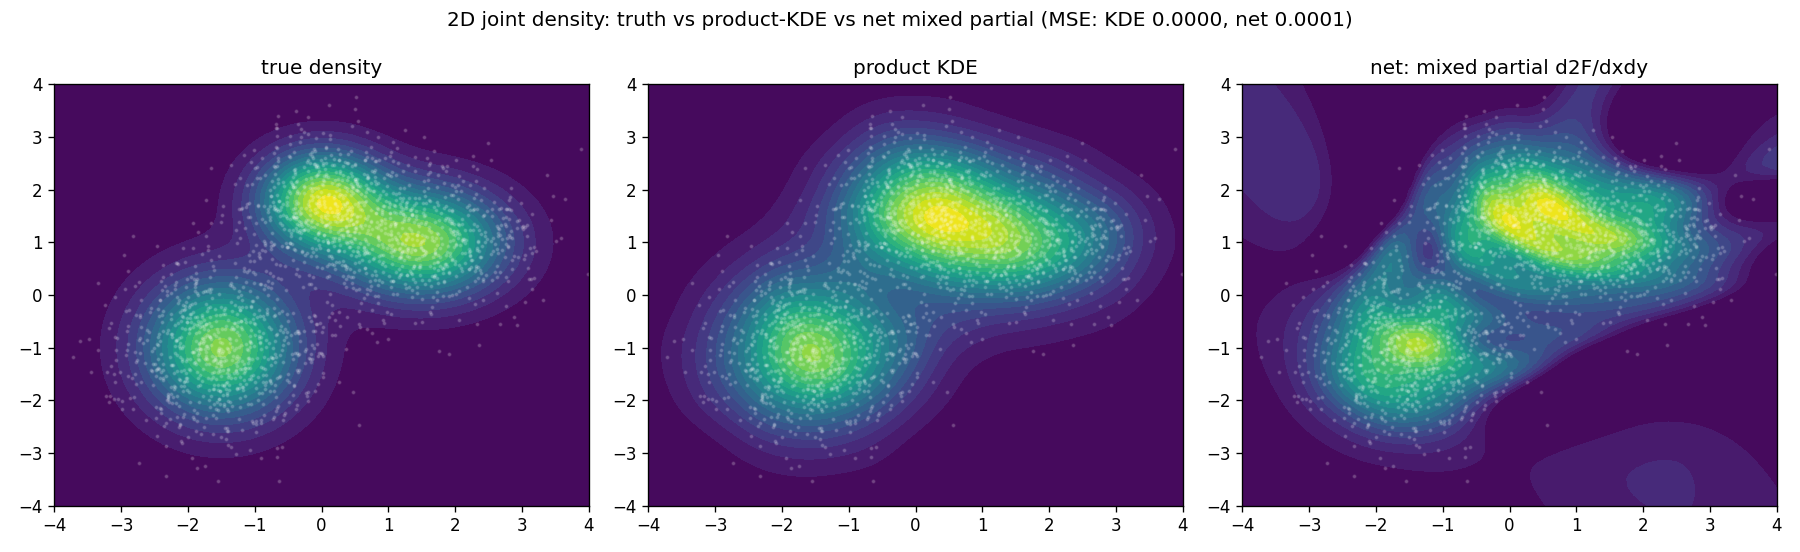
\includegraphics[width=\textwidth]{test_2d.png}
  \caption{Densita' congiunta 2D: verita', KDE prodotto, e derivata mista $\partial^2 F/\partial x
  \partial y$ della rete. La rete fornisce una densita' liscia e differenziabile con accuratezza pari
  alla KDE ($\mathrm{MSE}$ $0.00006$ contro $0.00004$) ma con interrogazione circa $157\times$ piu'
  veloce; la CDF empirica congiunta non e' derivabile a una densita' (solo picchi).}
\end{figure}

In due dimensioni la route CDF piu' derivata mista funziona bene. In \textbf{tre} dimensioni, pero', la
derivata terza della rete si degrada (MSE $4.3\times$ peggiore della KDE) e \textbf{non integra a $1$}
(integrale $1.70$, cioe' un errore di massa del $70\%$): la \textbf{monotonia $N$-crescente} (la
validita' di una CDF congiunta) non e' garantita dalla rettifica monovariata. Questo e' il vero nodo
aperto per il multivariato. Altre capacita' reali ma non esclusive: campionamento tramite CDF inversa
(un generatore compatto e monotono, la cui qualita' pero' pareggia Parzen), ed estrapolazione limitata
e sempre valida (garantita dalla sigmoide finale, pagata con l'offset di coda).

\section{Teoria e obiezione}

La CDF converge alla verita' a ritmo $n^{-1/2}$ in ogni dimensione (la maledizione della
dimensionalita' colpisce la \emph{densita'}, non la CDF); ma derivare $d$ volte una CDF stimata
riamplifica il rumore, cosicche' la difficolta' rientra sulla densita'. I metodi che davvero vincono la
maledizione (i normalizing flow) si addestrano a verosimiglianza diretta, non regredendo una KDE.
L'obiezione piu' forte: se si hanno i dati e liberta' di modellazione, un modello a verosimiglianza
diretta domina in accuratezza e mantiene ogni pregio strutturale.

\section{Verdetto: quando ha senso, quando no}

\paragraph{Ha senso quando valgono tutte:} si interroga la stima molte volte (si ammortizza
l'addestramento) o la si deve spedire o salvare compatta; si vuole un unico surrogato liscio,
differenziabile e monotono di una KDE di cui ci si fida; serve validita' garantita (massa $1$, non
negativa) senza penalita' di normalizzazione, specie in alta dimensione; non si puo' o non si vuole
fittare un modello a verosimiglianza diretto.

\paragraph{E' inutile quando ne vale anche una sola:} si vuole una stima \emph{migliore} (non puo'
battere il maestro); e' un problema one-shot o a poche interrogazioni (Parzen costa meno); si puo'
fittare un modello a verosimiglianza diretto (domina); servono code o quantili estremi accurati; una
KDE veloce risolve gia' il costo di interrogazione.

\section{Raccomandazione per il progetto}

Inquadrare il contributo onestamente come \textbf{distillazione e servizio}, non come stima: un MLP
sigmoidale regredisce fedelmente una CDF di Parzen in un surrogato compatto, a costo costante, valido
per costruzione e differenziabile, dichiarando esplicitamente che non batte in accuratezza il proprio
maestro. Guidare con i due vantaggi strutturali robusti (validita' gratuita della route CDF;
ammortamento e compressione), presentare l'economia della copula come risultato bidimensionale
condizionale, ed etichettare le capacita' come non esclusive. Non rivendicare che l'approccio batta la
maledizione della dimensionalita' per le densita'. Per il multivariato, dare priorita' alla monotonia
$N$-crescente, senza la quale la densita' congiunta via derivate miste non e' valida.

Il posizionamento piu' forte e onesto e' quello \emph{maestro-allievo}: e' cio' che si usa quando si
deve servire una KDE di cui ci si fida in modo economico, valido e differenziabile su larga scala.

\section*{Riferimenti}
\begin{itemize}\setlength{\itemsep}{0pt}
  \item Magdon-Ismail, M. e Atiya, A. (2002). Density Estimation and Random Variate Generation Using
  Multilayer Networks. \emph{IEEE Transactions on Neural Networks} 13(3).
  \item ``From CDF to PDF: A Density Estimation Method for High-Dimensional Data'', arXiv:1804.05316.
  \item ``Neural Likelihoods via Cumulative Distribution Functions'', arXiv:1811.00974.
\end{itemize}

\paragraph{Riproducibilita'.} Gli script e le figure sono in \texttt{temp\_analysis/}; il verdetto
verificato in \texttt{temp\_analysis/99\_verdict.md}, il piano e la ricerca in
\texttt{00\_plan\_and\_reflection.md} e \texttt{01\_research.md}.

\end{document}
